\documentclass[nojss]{jss}
\usepackage{thumbpdf,amsmath}
\newcommand{\PMTwoFive}{PM$_{2.5}$}

%%\VignetteIndexEntry{Caching and Distributing Statistical Analyses in R}
%%\VignetteDepends{cacher}

\author{Roger D. Peng\\
  Johns Hopkins Bloomberg School of Public Health}
\Plainauthor{Roger D. Peng}

\title{Caching and Distributing Statistical Analyses in \proglang{R}}
\Plaintitle{Caching and Distributing Statistical Analyses in R}

\Abstract{
  We present the \pkg{cacher} package for \proglang{R}, which provides
  tools for caching statistical analyses and for distributing these
  analyses to others in an efficient manner.  The \pkg{cacher} package
  takes objects created by evaluating \proglang{R} expressions and
  stores them in key-value databases.  These databases of cached
  objects can subsequently be assembled into packages for distribution
  over the web.  The \pkg{cacher} package also provides tools to help
  readers examine the data and code in a statistical analysis and
  reproduce, modify, or improve upon the results.  In addition,
  readers can easily conduct alternate analyses of the data.  We
  describe the design and implementation of the \pkg{cacher} package
  and provide two examples of how the package can be used for
  reproducible research.  This vignette was originally published
  as~\cite{peng:2008}
}

\Keywords{\proglang{R}, reproducible research, cached computation}
\Plainkeywords{R, reproducible research, cached computation}

\Volume{26}
\Issue{7}
\Month{July}
\Year{2008}
\Submitdate{2007-10-26}
\Acceptdate{2008-07-10}

\Address{
  Roger D. Peng\\
  Department of Biostatistics\\
  Johns Hopkins Bloomberg School of Public Health\\
  615 North Wolfe Street\\
  Baltimore MD 21205, United States of America\\
  E-mail:  \email{rpeng@jhsph.edu}\\
  URL:  \url{http://www.biostat.jhsph.edu/~rpeng/}
}

%% need no \usepackage{Sweave.sty}

\begin{document}

\section{Introduction}

Reproducible research is a phrase that is used to describe research
where the published results are accompanied by the software
environment and data used to produce these
results \citep{buck:dono:1995,schw:karr:clae:2000,gent:temp:2007}.
With the data and software, results can be recreated independently by
running the original analysis programs on the original data.
Reproduction is distinguished from replication in that replication
requires an independent investigator to obtain similar results using
new data and a comparable or identical analytic approach.  A minimum
requirement for reproducible research is that the data and computer
programs used to analyze the data are made available and distributed
to others \citep{peng:domi:zege:2006}.

The distribution of reproducible research is a problem for which the
solution varies depending on the complexity of the research.  Small
investigations involving moderately sized datasets and standard
computational techniques can be archived and distributed using
existing \textit{ad hoc} methods.  Readers can subsequently re-run the
entire analysis from start to finish to see if they can obtain the
same results as the authors.  Complex investigations involving large
or multiple linked datasets and sophisticated statistical computations
will be more difficult for readers to reproduce because of the
resources and time required for running the analysis.  In such a
situation a method is needed to give readers without equivalent
resources the ability to conduct an initial examination of the details
of the investigation and to reproduce or verify some of the results.

A framework in which reproducible research can be distributed using
\textit{cached computations} is described in \cite{peng:ecke:2007}.
Cached computations are results that are stored in a database as an
analysis is being conducted.  These stored results can be distributed
via websites or central repositories so that others may explore the
datasets and computer code for a given scientific investigation.

\begin{figure}[t!]
  \centering
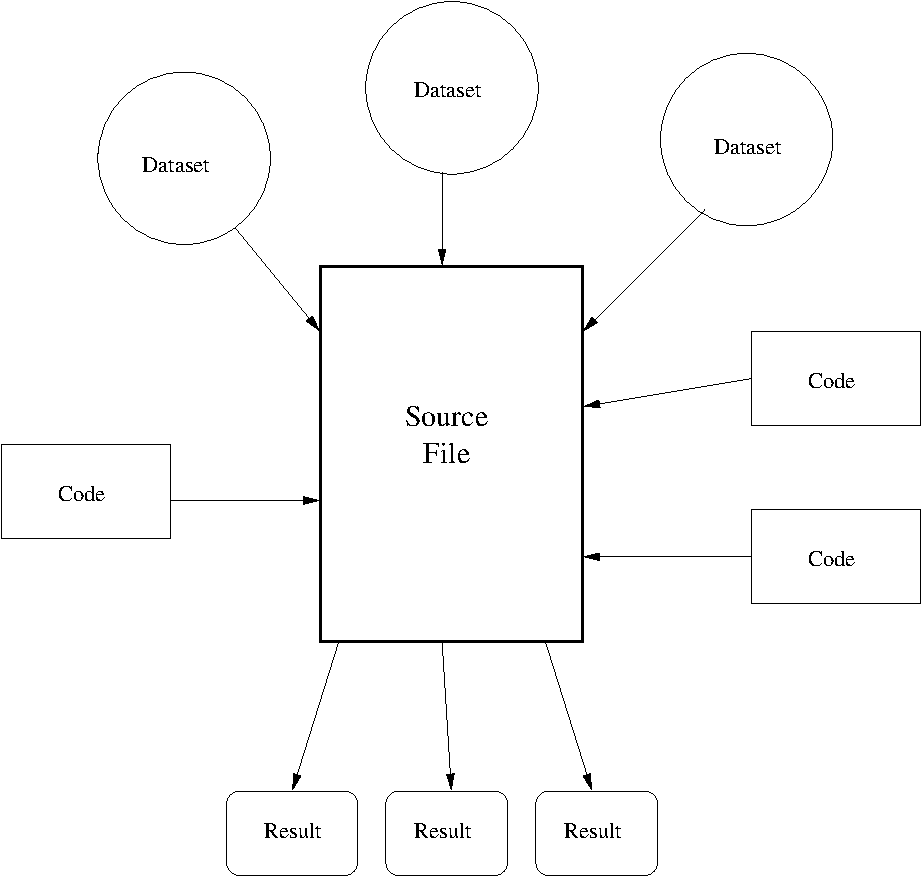
\includegraphics[width=4.8in]{model}
\caption{Conceptual model for the \pkg{cacher} package.}
\label{model}
\end{figure}

In this paper we describe in detail the design and implementation of
the \pkg{cacher} package, available from the Comprehensive \proglang{R}
Archive Network (CRAN) at \url{http://CRAN.R-project.org/package=cacher}.
It provides tools for caching arbitrary
statistical analyses and distributing them over the web.  We consider
statistical analyses as source files to be evaluated in a statistical
analysis environment such as \proglang{R}.  Theses source files serve
the purposes of reading in datasets, incorporating code from other
sources (e.g., loading other \proglang{R} packages, reading external
source files), executing analysis code, and producing results.  This
conceptual model is sketched in Figure~\ref{model}.
The \pkg{cacher} package caches the results produced along with any
datasets or external code that have been incorporated into the
analysis.  This way the reader can have access to those objects when
attempting to reproduce the analysis.


The idea of a ``compendium'' is described by \cite{gent:temp:2007} as
a way to publish a reproducible analysis by including multiple levels
of detail.  Readers with a casual interest in the paper may only read
the finished product while more interested readers can dig deeper into
the specifics of the data and computation.  The number of tools for
conducting reproducible research via compendiums in \proglang{R} and
other languages is generally increasing.  \proglang{R} users have
tools such as \code{Sweave} \citep{leis:2002} and \pkg{ESS}
\citep[Emacs Speaks Statistics,][]{ross:heib:spar:2004} to assist them in the
development of such compendiums as well as the \pkg{weaver}
package \citep{weaver:2007} and others \citep{peng:2007} for caching
computations.  Packages such as \pkg{SASWeave} \citep{lent:hojs:2007}
have emerged for literate programming using \proglang{SAS} and \LaTeX; for
non-\LaTeX\ users, the \pkg{odfWeave} package \citep{odfweave:2007} is
available for \proglang{R} users wishing to write documents in the
open document format (ODF, e.g., via \pkg{OpenOffice.org}).

The goal of the \pkg{cacher} package is to provide a means by which an
author  can assemble the code and data used in a statistical analysis
into a single package that can be distributed easily to others.  On
the receiving end the \pkg{cacher} package provides tools for readers
to evaluate an author's code and check to see if their results match
the original.  In addition, for very large analyses, the package
provides a mechanism by which readers can selectively reproduce
portions of an analysis that may be of interest without having to go
through the time-consuming process of reproducing the analysis in its
entirety.

The approach of the \pkg{cacher} package differs from previously
proposed approaches in that with the \pkg{cacher} package, code and
data are not linked to a human-readable document.  This approach has
both advantages and disadvantages.  While the ability of literate
programming approaches such as \code{Sweave} to provide a human-readable
document along with the code and data improves the reproducibility of
an analysis, the required knowledge of a markup language such as
\LaTeX, in addition to a programming language, can be a substantial
barrier for some analysts.  In particular, while \proglang{R} is used
in wide variety of fields to analyze data, \LaTeX\ is only used for
document preparation in a subset of those fields.  One aim of the
\pkg{cacher} package is to provide tools that are neutral towards
various document prepration methods, sacrificing some of the valued
added by the literate programming approaches.  Our approach is closer
in spirit to Jon Claerbout's model for reproducible
research \citep{schw:karr:clae:2000} than Donald Knuth's ``literate
programming'' model \citep{knut:1984}.

In Sections~\ref{sec:cacher}--\ref{sec:verify} we describe the basic
features of the \pkg{cacher} package.  Section~\ref{sec:examples}
provides examples of how the \pkg{cacher} package can be used to
cache, distribute, and verify statistical analyses.


\section{Caching statistical analyses}
\label{sec:cacher}

The \pkg{cacher} package provides interfaces for two types of users.
The first type consists of authors of statistical analyses who wish to
cache their analyses in a database and distribute the cached analysis
to others.  The second type of user consists of readers who wish to
obtain cached analyses over the web and explore the data and code in
those analyses.

The primary function in the \pkg{cacher} package for authors of
statistical analyses is the \code{cacher} function, which takes the
name of an \proglang{R} source file as its first argument.  This
should be a standard source file containing \proglang{R} code to be
evaluated and cached.  The remaining two arguments to \code{cacher}
specify the location of the cache directory (defaults to
\code{.cache}) and the log file (defaults to creating a log file in
the cache directory).

The simplest invocation of \code{cacher} is
\begin{Schunk}
\begin{Sinput}
R> library("cacher")
R> cacher("myanalysis.R")
\end{Sinput}
\end{Schunk}
where \code{myanalysis.R} is an \proglang{R} source file.  To print
log messages to the console, one can invoke
\begin{Schunk}
\begin{Sinput}
R> cacher("myanalysis.R", logfile = NA)
\end{Sinput}
\end{Schunk}
and obtain more information about what \code{cacher} is doing.

The basic procedure of \code{cacher} is to
\begin{enumerate}
\item
parse the \proglang{R} source file;
\item
create the necessary cache directories and subdirectories;
\item
set various configuration variables and hook functions for plotting
(see Section~\ref{sec:sideeffects});
\item
copy the source file to the cache directory;
\item
cycle through each expression in the source file:
\begin{enumerate}
\item
if an expression has never been evaluated, evaluate it and store any
resulting \proglang{R} objects in the cache database,
\item
if a cached result exists, lazy-load the results from the cache database,
\item
if an expression does not create any \proglang{R} objects (there is
nothing to cache), add the expression to the list of expressions where
evaluation needs to be forced,
\item
write out metadata for this expression to the metadata file.
\end{enumerate}
\end{enumerate}

The \code{cacher} function identifies each expression in a source file
by taking the SHA-1 digest of the expression, the expression history,
and the name of the source file.  The expression history is simply the
expression object containing every expression preceding the current
expression.  For the first expression, the expression history is of
length zero.  Using the expression history is a way to prevent
expressions such as
\begin{Schunk}
\begin{Sinput}
R> y <- x^2
\end{Sinput}
\end{Schunk}
from being inappropriately loaded from the cache.  Such an
expression may appear multiple times in a source file and we do not
want to load the same value for \code{y} every time since the value of
\code{x} may be changing.  Using the expression history can uniquely
identify each occurrence of a duplicate expression.

For each cached expression, a database file is created in the database
directory of the cache containing the serialized \proglang{R} objects
associated with that expression (if any).  If \code{cacher} encounters
an expression that has already been evaluated and for which objects
exist in the database, those objects will be lazy-loaded into the
user's workspace \citep[see e.g.,][]{rnews:ripley:2004}.  Hence, an
expression that has not been altered since a previous evaluation does
not need to be reevaluated---often loading objects from the cache will
be faster than reevaluating the expression.


\subsubsection{Metadata}

As the \code{cacher} function is running, it writes out metadata for
each expression to a metadata file in the cache directory.  This
metadata file is not used directly by the \code{cacher} function, but
it is used by the various other functions for exploring a cached
analysis (these functions are described in
Section~\ref{sec:exploring}).  Each source file processed by
\code{cacher} possesses its own metadata file and each entry of the
metadata file corresponds to an expression in the source file.  For
each expression, the metadata file contains a snippet of the
expression itself, the expression's SHA-1 digest, the names of any
\proglang{R} objects created by the expression, and whether evaluation
of the expression needs to be forced.


\subsubsection{Multiple source files}

As mentioned above, each expression in a source file is identified by
the digest of the expression itself, the expression history, and the
name of the source file.  The reason for including the name of the
source file is that a given cache directory can be used to process
multiple source files.  Since the same expression may occur in
different source files, it is important that we not load the value for
an expression associated with one file while processing another source
file.  In Section~\ref{sec:exploring} we describe how the user can
switch between exploring analyses from different source files using
the \code{sourcefile} function.

The \code{cacher} function identifies an analysis by the content of
the code file, not simply by the file name.  Therefore, two files with
the same name that contain different analyses will be treated
differently.  If \code{cacher} is used to process a file which has the
same name as an already processed analysis, then the new file will be
renamed in the cache so that it does not conflict with the existing
file.  Thus, if some changes are made to a file that \code{cacher} has
already seen, then it will treat the changed file as a new analysis.


\subsection{Expressions with side effects}
\label{sec:sideeffects}


Simple expressions, such as assignments, will typically result in a
single object being created in the global environment.  For example,
the expression
\begin{Schunk}
\begin{Sinput}
R> x <- 1:100
\end{Sinput}
\end{Schunk}
results in an object named \code{x} being created in the global
environment whose value is an integer sequence from 1 to 100.

However, there are other types of expressions which can result in
either multiple objects being created in the user's workspace or no
objects being created.  For example, the \code{source} function is
often used to load objects from an \proglang{R} code file.  Unless the
\code{local} argument is set to \code{TRUE}, these objects will by
default be created in the global environment.  When the \code{cacher}
function evaluates an expression that contains a call to
\code{source}, there will be objects created outside of the temporary
environment in which the expression is evaluated (again, unless the
argument \code{local = TRUE} is specified in the call to
\code{source}).  The \code{set.seed} function behaves in a similar way
by modifying (or creating) the \code{.Random.seed} object in the
global environment.

In order to handle the effects of functions like \code{source} the
function \code{evalAndCache}, which evalutes an expression and saves
the results to the cache database, first obtains a character vector of
the names of all the objects in the global environment.  After
evaluating the expression in a temporary environment, a check is made
to see if any new objects have been created or modified in the global
environment.  If so, those objects are saved to the database as well
as any objects that were created in the temporary environment.  Note
that we currently make a special case of the global environment.  If
the code being evaluated creates objects in some other environment,
then \code{cacher} will not be able to cache those objects.

Another example of a function with side effects is the \code{plot}
function (and related functions) from the \pkg{graphics} package.
Since \code{plot} does not create any objects in the global
environment, but rather creates a plot on a graphics device, there is
nothing for \code{cacher} to cache.  Currently, the approach of
\code{cacher} is to detect when a plot has been created by setting a
hook function for the \code{plot.new} function.  Each time
\code{plot.new} is called, an internal flag is set so that
\code{cacher} knows that evaluation of this expression needs to be
forced rather than cached.  We similarly set a hook function for
\code{grid.new} to detect the creation of \pkg{lattice} plots.

The \code{attach} function has a side effect which alters the elements
on the search list by adding a list, data frame, or saved workspace
file in the position specified.  The \code{cacher} function will
notice that no objects were created in the global environment or the
temporary environment and any call to \code{attach} will be flagged as
non-cacheable requiring evaluation.  If \code{cacher} is called
multiple times in the same session on a file containing an
\code{attach} call, then the corresponding object will be attached
(again) to the search list.  This may not be what the user intended.
Unfortunately, because it is not possible for \code{cacher} to know if
the external object being attached (e.g., a saved workspace file) has
changed, calls to \code{attach} must be evaluated every time.

There are many other types of expressions that have side effects and
do not result in the creation of objects in the global environment.
Expressions such as calls to \code{system} or functions which write
out files (e.g., \code{save}, \code{save.image}, \code{write.table},
\code{dput}, etc.) all result in objects being created outside of
\proglang{R}.  In general, these expressions cannot yet take advantage
of the caching mechanism in \pkg{cacher} and must be executed every
time \code{cacher} is run.

\section{Distributing a cached analysis over the web}
\label{sec:distribution}

Users who wish to distribute a cached statistical analysis over the
web and also have access to a local webserver, can post the cache
directory on the webserver so that others can download the materials
using the \code{clonecache} function.  All that is required is for the
user to copy the directory to a location on the webserver that is
visible to outside users.

The primary function for downloading a cached analysis is the
\code{clonecache} function.  The user can pass to \code{clonecache}
the URL of the directory containing a cached analysis.  Given a URL,
\code{clonecache} creates a cache directory on the user's local
machine and downloads the source files and metadata from the remote
machine.  By default, \code{clonecache} does not download any of the
database files since these could be very large and the user may not be
interested in every \proglang{R} object in the analysis.  In order to
force the downloading of all database objects when cloning, the user
needs to set \code{all.files = TRUE} when calling \code{clonecache}.
Once an analysis is cloned the functions described in
Section~\ref{sec:exploring} can be used to explore the code and data
objects in the analysis.


\section{Exploring a cached analysis}
\label{sec:exploring}


The \pkg{cacher} package provides some basic tools to allow users to
interact with the code and data provided in a cached analysis.  The
following functions make up the primary user interface for readers of
a cached analysis.
\begin{itemize}
\item
\code{showfiles}: Show what source files are available in the cache to
be examined by the user.  If the author of the package cached analyses
from multiple source files, then this function can be used to
determine which analysis should be examined.  One can switch between
different source files by calling the \code{sourcefile} function.
\item
\code{sourcefile}: Get or set the current source file for analysis.
\item
\code{code}: Show the expressions for a given source file.  By
default, \code{code} shows all expressions in a file in a one-line
abbreviated form along with their expression sequence numbers.  To see
each expression in its entirety, the argument \code{full = TRUE} must
be set.  If any expressions have been marked to be skipped by
\code{skipcode}, those expressions will be annotated with an asterisk.
\item
\code{showcode}: Show the original source file in the pager, which can
be useful if one is interested in seeing any comments.
\item
\code{loadcache}: Lazy-load cached computation databases into an
environment.  This function takes a numeric vector of expression
sequence numbers and loads objects associated with those expressions
in the order that the expressions are specified.  Once a cache
database is lazy-loaded, the object names appear in the environment
into which the database was loaded, but they do not occupy any memory
until they are first accessed.  If \code{loadcache} is used to load
objects from a remote cache (see Section~\ref{sec:distribution}), then
the corresponding database files will be downloaded on the object's
first access.
\item
\code{runcode}: This function takes as input a numeric vector of
expression sequence numbers executes the code in those expressions.
Each expression is evaluated in the order in which it appears in the
input vector.  By default, if a cached computation database is
associated with an expression, then the database is lazy-loaded via
\code{loadcache} rather than executed.  In order to force evaluation
of code in an expression, one needs to set \code{forceAll = TRUE} when
calling \code{runcode}.  If an error occurs when executing the code in
an expression, a message is printed to the console indicating the
error and the expression is skipped.  While the \code{runcode}
function can be used to evaluate individual expressions, the results
of such evaluation may not be correct if the dependent expressions
have not previously been evaluated.  In general, reproducible results
for a specific expression in an analysis can only be obtained by
evaluating all of the expressions in order up to that expression.
\item
\code{skipcode}: Force certain expressions to be skipped from
evaluation when using the \code{runcode} function (for example, if
certain external resources are not available).  There is a globally
maintained list of expressions that will be skipped for a given source
file.  If \code{num} is \code{NULL}, then the list of skipped
expressions is cleared.
\item
\code{showobjects}: Given an expression sequence number,
\code{showobjects} shows what objects were created (and hence cached)
by that expression.  These objects can subsequently be loaded into the
workspace with \code{loadcache}.  If \code{num} is a sequence, then a
single character vector is returned containing the union of the names
of the objects cached.
\end{itemize}





\section{Verifying an analysis}
\label{sec:verify}


The \pkg{cacher} package provides the \code{checkcode} function for
verifying the objects in a cached analysis.  A user who has downloaded
a cached analysis via \code{clonecache} or in some other manner can
verify a given \proglang{R} expression by evaluating the code on
his/her own machine and checking to see if the resulting object is
equivalent to the object stored in the database corresponding to that
expression.  The \code{checkcode} function takes a numeric vector of
expression sequence numbers and evaluates the corresponding
expressions while verifying that the resulting objects match the
cached objects.  The comparison of objects is done with the
\code{all.equal} function to allow for some minor differences, for
example, with floating point calculations.  Called with no arguments,
\code{checkcode} will check every expression in the source file.  If a
given expression does not have any \proglang{R} objects associated
with it, then there is nothing to check and \code{checkcode} moves to
the next expression.

When \code{checkcode} encounters an expression that cannot be
evaluated or where the computed object does not match the cached
object, a message is printed to the console indicating the problem.
In addition, \code{checkcode} will lazy-load the cached object into
the evaluation environment and continue checking subsequent
expressions in the source file.  Therefore, any expressions which
depend on the object corresponding to the non-verified expression will
use the cached object rather than the computed one.

For example, an analysis will typically contain an expression which
reads in a dataset using a function such as \code{load} or
\code{read.table}.  These functions read data from external
connections (usually files) and load them into the user's workspace.
If the user does not also have possession of these external files,
then there is no way for the user to verify the evaluation of that
expression.  However, the data from the file is nevertheless cached in
the database so it is possible to evaluate subsequent expressions
based on the cached version of the data.
Section~\ref{sec:exampleverify} gives an example of how
\code{checkcode} handles this particular situation.


\subsection{Verifying the integrity of objects}

In addition to comparing the output of evaluating code with cached
objects, one can check the integerity of the cached objects to make
sure that there has not be any corruption to the files (particularly,
when being transferred over the network).  Each object stored in the
cache has with it the SHA-1 digest of the object itself.  The
\code{checkobjects} function can be used to compare this SHA-1 digest
with the digest of the object.  Any corruption of the data will result
in a mismatch between the stored digest and computed digest.

\section{Examples}
\label{sec:examples}

\subsection{Basic usage}



To illustrate some of the features of the \pkg{cacher} package we will
use the following simple statistical analysis of the \code{airquality}
dataset from the \pkg{datasets} package which comes with \proglang{R}.  The code
for the entire analysis is printed below.
\begin{Schunk}
\begin{Soutput}
library("datasets")
library("stats")

data("airquality")

fit <- lm(Ozone ~ Wind + Temp + Solar.R, data = airquality)
summary(fit)

## Plot some diagnostics
par(mfrow = c(2, 2))
plot(fit)

## Interesting non-linear relationship
temp <- airquality$Temp
ozone <- airquality$Ozone

par(mfrow = c(1, 1))
plot(temp, ozone)
\end{Soutput}
\end{Schunk}
The code is contained in a file called ``\code{sample.R}'' which comes with
the \pkg{cacher} package.  The above analysis is fairly simple and not
very time-consuming so it is easily reproduced by anyone who can run
R, without any need for caching.  Nevertheless, it is useful for
demonstrating how the \pkg{cacher} package works.

The first step is to install the \pkg{cacher} package from the
CRAN and load it into \proglang{R}.
\begin{Schunk}
\begin{Sinput}
R> library("cacher")
R> options(width = 60)
R> setConfig("verbose", TRUE)
\end{Sinput}
\end{Schunk}
For now, we also set the global \code{verbose} option to be
\code{TRUE}, making \code{cacher} be somewhat more ``chatty'' (the
default is \code{FALSE}).

The \code{cacher} function accepts a file name as its first argument.
This file should contain the code for the analysis that you want to
cache.  Other arguments include the name of the cache directory
(defaults to \code{.cache}) and the name of the log file (defaults to
\code{NULL}).  If \code{logfile = NULL} then messages will be printed
to a file in the cache directory.  Setting \code{logfile = NA} will
send messages to the console.

The ``\code{sample.R}'' file containing the above analysis comes with the
\pkg{cacher} package and can be copied into your working directory.
Given a file containing the code of an analysis, you can call the
\code{cacher} function as
\begin{Schunk}
\begin{Sinput}
R> cacher("sample.R")
\end{Sinput}
\begin{Soutput}
creating cache directory '.cache'

Call:
lm(formula = Ozone ~ Wind + Temp + Solar.R, data = airquality)

Residuals:
    Min      1Q  Median      3Q     Max 
-40.485 -14.219  -3.551  10.097  95.619 

Coefficients:
             Estimate Std. Error t value Pr(>|t|)
(Intercept) -64.34208   23.05472  -2.791  0.00623
Wind         -3.33359    0.65441  -5.094 1.52e-06
Temp          1.65209    0.25353   6.516 2.42e-09
Solar.R       0.05982    0.02319   2.580  0.01124

Residual standard error: 21.18 on 107 degrees of freedom
  (42 observations deleted due to missingness)
Multiple R-squared: 0.6059,	Adjusted R-squared: 0.5948 
F-statistic: 54.83 on 3 and 107 DF,  p-value: < 2.2e-16 
\end{Soutput}
\end{Schunk}
The \code{cacher} function evaluates each expression in the file and
prints any resulting output to the console.  For example, the summary
of the fitted linear model is printed to the console while the two
plots are sent to the appropriate graphics device.  The log messages
are written to a file in \code{.cache/log/sample.R.log} which
contains information about each expression evaluated by \code{cacher}.
We will discuss the contents of the log file in
Section~\ref{sec:logfile}.

When cacher evaluates each code expression, the results of the
evaluation are cached to the database and lazy-loaded back into the
workspace.  After running the ``\code{sample.R}'' analysis, we can see that
there are the following objects now in the workspace:
\begin{Schunk}
\begin{Sinput}
R> ls()
\end{Sinput}
\begin{Soutput}
[1] "airquality" "fit"        "ozone"      "temp"      
\end{Soutput}
\end{Schunk}
Since the objects are lazy-loaded, they do not occupy any memory
until they are accessed.  The lazy-loading is not as important on the
first evaluation but can reduce the amount of evaluation time required
on subsequent analysis

For example, take the following very simple set of expressions.
\begin{Schunk}
\begin{Soutput}
x <- rnorm(1000000)
s <- summary(x)
print(s)
\end{Soutput}
\end{Schunk}
The first expression creates a vector of 1 million standard Normal
random variates and the second computes a summary (a five-number
summary plus the mean).  The amount of time to evaluate these
expressions the first time is
\begin{Schunk}
\begin{Sinput}
R> systime <- system.time(cacher("bigvector.R"))
\end{Sinput}
\begin{Soutput}
       Min.     1st Qu.      Median        Mean     3rd Qu. 
-5.12300000 -0.67230000  0.00003428  0.00049710  0.67530000 
       Max. 
 4.66300000 
\end{Soutput}
\begin{Sinput}
R> print(systime)
\end{Sinput}
\begin{Soutput}
   user  system elapsed 
  1.756   0.400   2.164 
\end{Soutput}
\end{Schunk}
In this case, the evaluation time is about
1.8 seconds.  After running
\code{cacher}, the objects \code{x} and \code{s} reside in the
workspace and have been cached to the database.  Subsequent
evaluations of the same code should take much less time since we can
simply load \code{x} and \code{s} from the cache.
\begin{Schunk}
\begin{Sinput}
R> rm(x, s)
R> systime <- system.time(cacher("bigvector.R"))
\end{Sinput}
\begin{Soutput}
       Min.     1st Qu.      Median        Mean     3rd Qu. 
-5.12300000 -0.67230000  0.00003428  0.00049710  0.67530000 
       Max. 
 4.66300000 
\end{Soutput}
\begin{Sinput}
R> print(systime)
\end{Sinput}
\begin{Soutput}
   user  system elapsed 
  0.028   0.000   0.027 
\end{Soutput}
\end{Schunk}
Now the evaluation only takes about
0.028 seconds.  In fact, the
analysis here is particularly quick because we do not need the
\code{x} vector at all.  We can simply print the summary object
\code{s}.

Even if we did need to access the vector \code{x}, loading from the
cache is often faster than regenerating all of the random Normals
using \code{rnorm}.  For example, if we wanted to calculate the 95th
percentile of the data, then we could simply do
\begin{Schunk}
\begin{Sinput}
R> systime <- system.time(q95 <- quantile(x, 0.95))
R> print(q95)
\end{Sinput}
\begin{Soutput}
     95% 
1.644256 
\end{Soutput}
\begin{Sinput}
R> print(systime)
\end{Sinput}
\begin{Soutput}
   user  system elapsed 
  0.492   0.028   0.520 
\end{Soutput}
\end{Schunk}



\subsubsection{Exploring a cached analysis}


Once an analysis has been cached using \code{cacher}, it can be
explored using the utilities provided in the \pkg{cacher} package.
Since you can cache analyses from multiple files (as we have done
above), we can show which analyses have already been cached using the
\code{showfiles} function.
\begin{Schunk}
\begin{Sinput}
R> showfiles()
\end{Sinput}
\begin{Soutput}
[1] "sample.R"    "bigvector.R"
\end{Soutput}
\end{Schunk}
Here we see the file names corresponding to the two files that we
analyzed in the previous section.  If you want to examine a particular
analysis, you can use the \code{sourcefile} function to choose that
analysis and \code{showcode} will simply display the raw source file.
\begin{Schunk}
\begin{Sinput}
R> sourcefile("bigvector.R")
R> showcode()
\end{Sinput}
\begin{Soutput}
x <- rnorm(1000000)
s <- summary(x)
print(s)
\end{Soutput}
\end{Schunk}
You can also use the \code{code} function to display the code in a
summary form
\begin{Schunk}
\begin{Sinput}
R> sourcefile("sample.R")
R> code()
\end{Sinput}
\begin{Soutput}
source file: sample.R
1  library("datasets")
2  library("stats")
3  data("airquality")
4  fit <- lm(Ozone ~ Wind + Temp + 
5  summary(fit)
6  par(mfrow = c(2, 2))
7  plot(fit)
8  temp <- airquality$Temp
9  ozone <- airquality$Ozone
10  par(mfrow = c(1, 1))
11  plot(temp, ozone)
\end{Soutput}
\end{Schunk}
The \code{code} function truncates expressions to a single line and
also shows the sequence number assigned to each expression in the
order that the expression is encountered in the source file.  In order
to see the full code for each expression, you can set the \code{full =
TRUE} option to \code{code}.

The first thing you might do when exploring a cached analysis is to
explore the elements of the cache database itself.  You can list the
objects available using the \code{showobjects} function, which returns
a character vector of the names of each object in the database.
Passing an expression sequence number to \code{showobjects} via the
\code{num} argument shows the objects created by that expression.
\begin{Schunk}
\begin{Sinput}
R> showobjects()
\end{Sinput}
\begin{Soutput}
[1] "airquality" "fit"        "temp"       "ozone"     
\end{Soutput}
\begin{Sinput}
R> showobjects(8)
\end{Sinput}
\begin{Soutput}
[1] "temp"
\end{Soutput}
\begin{Sinput}
R> showobjects(1)
\end{Sinput}
\begin{Soutput}
character(0)
\end{Soutput}
\end{Schunk}
These objects can be lazy-loaded into the workspace using the
\code{loadcache} function.
\begin{Schunk}
\begin{Sinput}
R> loadcache()
R> ls()
\end{Sinput}
\begin{Soutput}
[1] "airquality" "fit"        "ozone"      "temp"      
\end{Soutput}
\end{Schunk}
Now, we can print the linear model fit (without actually fitting the
model) by calling
\begin{Schunk}
\begin{Sinput}
R> print(fit)
\end{Sinput}
\begin{Soutput}
Call:
lm(formula = Ozone ~ Wind + Temp + Solar.R, data = airquality)

Coefficients:
(Intercept)         Wind         Temp      Solar.R  
  -64.34208     -3.33359      1.65209      0.05982  
\end{Soutput}
\end{Schunk}
The \code{loadcache} function takes a \code{num} argument which can be
a vector of indices indicating code expression sequence numbers.  For
example, if you want to load only the objects associated with
expression 4 (i.e., the \code{fit} object), then you can call
\code{loadcache(4)}.

In addition to exploring the objects in the cache database, you may
wish to run the analysis on your own computer for the purposes of
reproducing the original results.  You can run individual expressions
or a sequence of expressions with the \code{runcode} function.  The
\code{runcode} function accepts a number or a sequence of numbers
indicating expressions in an analysis.  For example, in order to run
the first four expressions in the ``\code{sample.R}'' analysis, we could call
\begin{Schunk}
\begin{Sinput}
R> rm(list = ls())
R> code(1:4)
\end{Sinput}
\begin{Soutput}
source file: sample.R
1  library("datasets")
2  library("stats")
3  data("airquality")
4  fit <- lm(Ozone ~ Wind + Temp + 
\end{Soutput}
\begin{Sinput}
R> runcode(1:4)
\end{Sinput}
\begin{Soutput}
evaluating expression 1
evaluating expression 2
loading cache for expression 3
loading cache for expression 4
\end{Soutput}
\begin{Sinput}
R> ls()
\end{Sinput}
\begin{Soutput}
[1] "airquality" "fit"       
\end{Soutput}
\end{Schunk}
In this case, expressions 1 and 2 are evaluated but expressions 3
and 4 are loaded from the cache.  By default, \code{runcode} does not
evaluate expressions for which it can load the results from the cache.
In order to force evaluation of all expressions, you need to set the
option \code{forceAll = TRUE}.



\subsubsection{Understanding the log file}
\label{sec:logfile}

As each expression is being evaluated, \code{cacher} keeps track of
which expressions result in the creation of new objects (including
modification of existing objects) and which expressions have side
effects.  Expressions with side effects cannot be cached and therefore
must always be evaluated.  The primary operation falling into this
category is plotting, which launches a graphics device and makes
changes to that device.  One exception is \pkg{lattice} plots which
can be stored as objects and therefore cached.  The log file contains
information about each expression and whether it needs to force
evaluation.  Here we print the first few lines of the log file for
this analysis.

\begin{Schunk}
\begin{Soutput}
1: library("datasets")
  eval expr and cache
  expression has side effect: f92adaa84e2ae7800e91ee5fead3a3db06d18f9a
2: library("stats")
  eval expr and cache
  expression has side effect: 223a036ba6a2561e5c23716840e9090670824ff4
3: data("airquality")
  eval expr and cache
4: fit <- lm(Ozone ~ Wind + Temp + 
  eval expr and cache
5: summary(fit)
  eval expr and cache
\end{Soutput}
\end{Schunk}
Understanding the log file output is not critical to using
\code{cacher} but it is occasionally useful to know what the function
is doing for a given expression.  Each expression is assigned a number
based on when it is encountered in the source file and a snippet of
the expression is printed immediately after the number.  Below,
\code{cacher} will indicate if the expression needs to be evaluated
and cached and will try to determine if the expression resulted in a
side effect.  The check for side effects is rudimentary and will not
catch all cases.  Once the expression has been cached, \code{cacher}
will reload the results from the cache into the global environment
(i.e., workspace) and move to the next expression.

Running the analysis a second time with \code{cacher} results in the
following log file being generated.
\begin{Schunk}
\begin{Soutput}
1: library("datasets")
  -- loading expr from cache
2: library("stats")
  force expression evaluation
3: data("airquality")
  -- loading expr from cache
4: fit <- lm(Ozone ~ Wind + Temp + 
  -- loading expr from cache
\end{Soutput}
\end{Schunk}
Here we see that expressions 1 and 2 were forced to be evaluated
because the \code{library} function results in a side effect
(i.e., altering the search list).  Expressions 3 and 4 create objects
in the workspace so they can be lazy-loaded from the cache.  Note here
that although the \code{airquality} dataset is loaded from the cache,
it is not needed if you are primarily interested in examining the
\code{fit} object from the \code{lm} call.  This is where lazy-loading
is very useful.  However, if you want to fit a different model, say,
with some interactions, then of course the original data will be
loaded into the workspace the first time it is accessed.


\subsubsection{Posting a cache directory}


If you have access to a webserver you can post your cache directory
directly on the webserver for others to access.  Once made available
on a webserver, others can access your cache directory by using the
\code{clonecache} function in the \pkg{cacher} package and the URL of
the directory on your webserver.  For example, we can download the
analysis corresponding to the ``\code{bigvector.R}'' file by calling
\begin{Schunk}
\begin{Sinput}
R> clonecache("http://penguin.biostat.jhsph.edu/bigvector.cache")
\end{Sinput}
\begin{Soutput}
created cache directory '.cache'
downloading source file list
downloading metadata
downloading source files
downloading cache database file list
\end{Soutput}
\end{Schunk}
This call to \code{clonecache} downloads all of the relevant cache
files related to the analysis except for the cache database files.  In
order to download the cache database files, the option \code{all.files
= TRUE} must be set.

Once a cache package has been downloaded using \code{clonecache} you
can use all of the tools described in the previous sections to explore
the cache and the run some of the analyses.
\begin{Schunk}
\begin{Sinput}
R> showfiles()
\end{Sinput}
\begin{Soutput}
[1] "bigvector.R"
\end{Soutput}
\begin{Sinput}
R> sourcefile("bigvector.R")
R> code()
\end{Sinput}
\begin{Soutput}
source file: bigvector.R
1  x <- rnorm(1000000)
2  s <- summary(x)
3  print(s)
\end{Soutput}
\begin{Sinput}
R> showobjects()
\end{Sinput}
\begin{Soutput}
[1] "x" "s"
\end{Soutput}
\begin{Sinput}
R> loadcache()
R> print(s)
\end{Sinput}
\begin{Soutput}
/ transferring cache db file d7952a4732ffa55c045958205340...
      Min.    1st Qu.     Median       Mean    3rd Qu. 
-4.6570000 -0.6737000  0.0006063  0.0012460  0.6755000 
      Max. 
 5.1400000 
\end{Soutput}
\end{Schunk}
By default, \code{clonecache} does not download the cache database
files until they are needed in order to minimize the amount of data
that is transferred.  Cache database files are only transferred from
the remote host when the objects associated with them are first
accessed.

In the above example, the database file corresponding to the object
\code{s} is only transferred when we call \code{print(s)}.  When a
database object has to be downloaded from the remote site, a message
will be printed to the screen indicating the transfer.




\subsubsection{Verifying a cached analysis}
\label{sec:exampleverify}

Once you have cloned an analysis conducted by someone else, you may
wish to verify that the computation that you run on your computer
leads to the same results that the original author obtained on his/her
computer.  This can be done with the \code{checkcode} function.  The
\code{checkcode} function essentially evaluates each expression
locally (if it can) and compares the output with the corresponding
value stored in the cache database.

If the locally created object and the cached object are the same, then
that expression is considered verified.  If an expression does not
create any objects, then there is nothing to compare.  If the locally
created object and the cached object are different, the the
verification fails and \code{checkcode} will indicate which objects it
could not verify.

For example, we can run the \code{checkcode} function on the analysis
of the \code{airquality} dataset from before.  Here we will only check
the first four code expressions.
\begin{Schunk}
\begin{Sinput}
R> unlink(".cache", recursive = TRUE)
R> clonecache("http://penguin.biostat.jhsph.edu/combined.cache")
\end{Sinput}
\begin{Soutput}
created cache directory '.cache'
downloading source file list
downloading metadata
downloading source files
downloading cache database file list
downloading metadata
downloading source files
downloading cache database file list
\end{Soutput}
\begin{Sinput}
R> sourcefile("sample.R")
R> showobjects(1:4)
\end{Sinput}
\begin{Soutput}
[1] "airquality" "fit"       
\end{Soutput}
\begin{Sinput}
R> checkcode(1:4)
\end{Sinput}
\begin{Soutput}
evaluating expression 1
evaluating expression 2
checking expression 3
/ transferring cache db file 142d241ba5b4fbb5646a189fce5c...
+ object 'airquality' OK
checking expression 4
/ transferring cache db file ad5720cbda29135e8412d130a6de...
+ object 'fit' OK
\end{Soutput}
\end{Schunk}
In the first four expressions, there are two objects created: the
dataset \code{airquality} and the linear model object \code{fit}.  The
\code{checkcode} function compares each of those objects with the
version stored in the cache database (which we previously cloned from
the web).  In this case, the objects match and the computations are
verified.  Notice that in expression 3, the database file for the
\code{airquality} object had to be downloaded so that it could be
checked against the locally created version.

We can check the code in the ``\code{bigvector.R}'' analysis also.  In this
analysis there are two objects that need to be verified: \code{x}, the
vector of standard normals and \code{s} the ``summary'' object.
\begin{Schunk}
\begin{Sinput}
R> sourcefile("bigvector.R")
R> checkcode()
\end{Sinput}
\begin{Soutput}
checking expression 1
/ transferring cache db file fb877f8375799370cef47fce86a9...
- object 'x' not verified, FAILED
- Mean relative difference: 1.414418
checking expression 2
/ transferring cache db file d7952a4732ffa55c045958205340...
- object 's' not verified, FAILED
- Mean relative difference: 0.02266224
evaluating expression 3
      Min.    1st Qu.     Median       Mean    3rd Qu. 
-5.1260000 -0.6762000  0.0020960  0.0002266  0.6750000 
      Max. 
 4.6490000 
\end{Soutput}
\end{Schunk}
Notice that expressions 1 and 2 failed for a common reason
(expression 3 had no objects to verify).  Since the analysis did not
set the random number generator seed in the beginning, the generation
of the Normal random variates on the local machine is not the same as
that for the original analysis.  Therefore, the object \code{x} is not
reproducible (nor is \code{s}).

Of course, there are limitations to verifying statistical analyses.
Analyses may take a long time to run and therefore it may take a long
time to verify a given computation.  If one does not have the
necessary external resources (i.e., hardware, software) then it may not
be possible to verify an analysis at all.  Currently, verification of
analyses is limited to \proglang{R} objects only.  We cannot verify the output of
summary or print functions nor can we verify plots (although lattice
plots can be verified if they are stored as \proglang{R} objects).

Certain analyses may load external datasets or inputs which will
generally not be available to the other users.  A typical analysis
might be of the form
\begin{Schunk}
\begin{Soutput}
data <- read.csv("faithful.csv")
with(data, plot(waiting, eruptions))

library("splines")
fit <- lm(eruptions ~ ns(waiting, 4), data = data)

xpts <- with(data, seq(min(waiting), max(waiting), len = 100))
lines(xpts, predict(fit, data.frame(waiting = xpts)))
\end{Soutput}
\end{Schunk}
This analysis reads in the the ``Old Faithful'' dataset which
contains eruption times and waiting periods for the Old Faithful
geyser in Yellowstone National Park.  Although this dataset is
available from the \proglang{R} installation, we have exported it here to a
comma-separated-value file for demonstration.

The original author of this analysis can run the \code{cacher}
function on this analysis file and distributed it to others.
\begin{Schunk}
\begin{Sinput}
R> cacher("faithful.R")
\end{Sinput}
\end{Schunk}
However, another user (presumably on a different computer) will not be
able to verify all of the code in this analysis
\begin{Schunk}
\begin{Sinput}
R> sourcefile("faithful.R")
R> checkcode()
\end{Sinput}
\begin{Soutput}
checking expression 1
- problem evaluating expression, FAILED
- simpleWarning: cannot open file 'faithful.csv': No
- such file or directory
- loading objects from cache
/ transferring cache db file 255fb954f855b0e53bafa43091fc...
evaluating expression 2
evaluating expression 3
checking expression 4
/ transferring cache db file a15033591616f8a9b693ca1e4faf...
+ object 'fit' OK
checking expression 5
/ transferring cache db file bed8272d401434750a5c0c4c47ce...
+ object 'xpts' OK
evaluating expression 6
\end{Soutput}
\end{Schunk}
Here, the first expression, which reads the dataset in via
\code{read.csv} cannot be verified because the ``\code{faithful.csv}'' file
is not available.  However, the other expressions can be run on the
local machine and are verifiable since they can use the cached copy of
the dataset.

\subsection{Conducting an alternate analysis}
\label{sec:exampleusage2}


In this section we will illustrate the use of the \pkg{cacher} package
to reproduce some results from a large epidemiological study of the
health effects of fine particulate matter air pollution.  This study
was a multi-site time series study examining the short-term
relationship between particulate matter $\leq 2.5 \mu$m in aerodynamic
diameter (\PMTwoFive) and daily hospital admission rates for various
cardiovascular and respiratory diseases~\citep{mcaps:2006}.

This study produced a county-specific estimate of the log relative
risk relating increases in daily \PMTwoFive\ with daily hospital
admission rates.  These risks can be found at the study's website at
http://www.biostat.jhsph.edu/MCAPS/.  Below, we present a sensitivity
analysis of these log relative risks and demonstrate how they can be
pooled together to obtain a ``national average'' risk estimate using a
two-level Normal hierarchical model~\citep[more details
in][]{domi:same:zege:2000}.


First, we can clone the cached analysis by calling \code{clonecache}.
\begin{Schunk}
\begin{Sinput}
R> library("cacher")
R> options(width = 60)
R> clonecache("http://penguin.biostat.jhsph.edu/mcaps.cache")
\end{Sinput}
\begin{Soutput}
created cache directory '.cache'
downloading source file list
downloading metadata
downloading source files
downloading cache database file list
\end{Soutput}
\end{Schunk}
Here we see that there is only one source file available, the
\code{mcaps.R} file.  
\begin{Schunk}
\begin{Sinput}
R> showfiles()
\end{Sinput}
\begin{Soutput}
[1] "mcaps.R"
\end{Soutput}
\begin{Sinput}
R> sourcefile("mcaps.R")
\end{Sinput}
\end{Schunk}
We can list the code expressions with the \code{code} function.
\begin{Schunk}
\begin{Sinput}
R> code(1:7)
\end{Sinput}
\begin{Soutput}
source file: mcaps.R
1  Sys.setlocale(locale = "C")
2  estimates <- read.csv("http://www.biostat.jhsph.edu/MC...
3  estimates <- transform(estimates, 
4  library("tlnise")
5  HF <- subset(estimates, outcome == 
6  initTLNise()
7  pooled <- with(HF, tlnise(beta, 
\end{Soutput}
\end{Schunk}

The first six code expressions read the data from the website and pool
the risk estimaets for heart failure across the 202 counties in the
study.  For the pooling, we use Phil Everson's \pkg{TLNise}
software~\citep{ever:morr:2000}, an \proglang{R} version of which is
available on CRAN \citep{tlnise}.  The first thing we can do is the verify that we
are capable of producing the same results that the original authors
did.  The \code{checkcode} function can be used to check the first six
expressions.
\begin{Schunk}
\begin{Sinput}
R> checkcode(1:7)
\end{Sinput}
\begin{Soutput}
evaluating expression 1
checking expression 2
/ transferring cache db file d33bf70c06481a745ebfd57a0f0e...
+ object 'estimates' OK
checking expression 3
/ transferring cache db file 0d389a6f8121c60b66c13389cf3a...
+ object 'estimates' OK
evaluating expression 4
Two-level normal independent sampling estimation
(version 0.2-7)
checking expression 5
/ transferring cache db file 48dc3abbde978864d5ea447038de...
+ object 'HF' OK
evaluating expression 6
checking expression 7
/ transferring cache db file 51999c8bd7db146ebe049d4fb4de...
+ object 'pooled' OK
\end{Soutput}
\end{Schunk}
Here we see that the six expressions were evaluated properly and the
objects created matched those created by the original authors.
Database objects were downloaded from the archive as needed.

The original pooled national average log relative risk for
hospitalization for heart failure can be found by loading the cached
objects for expression 7.
\begin{Schunk}
\begin{Sinput}
R> loadcache(7)
R> pooled$gamma
\end{Sinput}
\begin{Soutput}
          est           se   est/se
0 0.001291823 0.0002505152 5.156663
\end{Soutput}
\end{Schunk}
This risk estimate shown in the \code{est} column can be interpreted
as a 1.29\% increase in
admissions of heart failure associated with a 10 $\mu$g/m$^3$ increase
in ambient \PMTwoFive.

One important issue in this analysis is the sensitivity of the
Bayesian hierarchical model to the specification of the prior
distribution.  In particular, the TLNise software places a uniform
prior on the second-level covariance matrix, sometimes referred to as
the heterogeneity matrix, which describes the natural variation of the
relative risks across counties.  Since the original authors used the
default settings, it is of interest to see if the national average
estimates vary when this prior specification is altered.

The \code{tlnise} function has an option called \code{prior} which can
be used to change the nature of the prior distribution on the
second-level covariance matrix.  Here we try two alternate priors.
First, we need to call \code{loadcache} first in order to obtain the
data frame \code{HF}.
\begin{Schunk}
\begin{Sinput}
R> loadcache(1:7)
R> library("tlnise")
R> p0 <- with(HF, tlnise(beta, var, prnt = FALSE, 
+     prior = 0))
R> p2 <- with(HF, tlnise(beta, var, prnt = FALSE, 
+     prior = 2))
\end{Sinput}
\end{Schunk}
We can now compare the estimates obtained using the two alternative
prior specifications with the original estimates
\begin{Schunk}
\begin{Sinput}
R> rbind(p0$gamma, p2$gamma, pooled$gamma)
\end{Sinput}
\begin{Soutput}
          est           se   est/se
0 0.001293042 0.0002507844 5.155989
0 0.001293785 0.0002517023 5.140142
0 0.001291823 0.0002505152 5.156663
\end{Soutput}
\end{Schunk}
Here we see that there is some variation between the estimates but the
estimates are qualitatively similar.


\section{Discussion and future work}

Currently, authors can use the \pkg{cacher} package to cache an
analysis and distribute the analysis over the web.  The package
provides readers tools for downloading these cached analyses and
exploring the code and data within them.  The \pkg{cacher} package is
limited in that it cannot take advantage of the extra information
provided in the literate programming context.  For example, the
\pkg{cacheSweave} and \pkg{weaver} packages organize code by the
``chunks'' defined in the combined \proglang{R}/\LaTeX\ document.  The
code chunks can provide extra information about the context of a set
of code expressions.  For example, it is possible to find out whether
a figure is being produced.  Without the existence of code chunks, the
\pkg{cacher} package must evaluate evaluate each code expression
individually.

Plotting in general is currently a weak spot in the \pkg{cacher}
package.  While hooks are used to detect when plotting occurs in an
expression so that those expressions can be flagged as non-cacheable,
better approaches are needed.  For example, it may be of use to cache
the graphics files (if any are produced) or to save the output of
screen device to a file.  Recent developments in \proglang{R} may
allow this to be done in a more convenient manner.

The handling of side effects is another area in need of further
development.  While \pkg{cacher} tries to handle some basic cases and
works reasonably well in standard usages, it will not create an
accurate cache in more complex situations, particularly if things like
external pointers or environments are used extensively.  Experience
will help to gauge the demand for handling such objects and new cases
will need to be handled as the need arises.

One possible direction for future work is to provide the ability to
annotate the code in a source file.  Such annotations could provide
hints to \code{cacher} regarding what the code is doing.  For example,
if a set of expressions gives rise to a figure (e.g., a PDF file), then
we can associate that set of expressions with the figure and give the
reader more information about the analysis via the reader tools.
Similar annotations could be provided for tables and other results
that the author deems interesting.  This way, a reader interested in
particular table/figure of results could quickly identify the segment
of code that produced the results.

Another area for further development includes providing tools to help
readers edit cached analyses and to integrate their modifications into
the original computations.  Currently, the reader tools are
``read-only'', allowing readers to examine and explore an analysis,
but not allowing them to edit the original source file.  For example,
in order to test the sensitivity of an analysis to a set of
assumptions (as in Section~\ref{sec:exampleusage2}), a reader might
want to alter a specific group of \proglang{R} expressions and re-run
the entire analysis with the altered expressions.

Currently, only \proglang{R} users can interact with the data and code
in cache directories that have been posted to the web (i.e., via the
\pkg{cacher} package's \code{clonecache} function).  It might be
desirable to provide a more useful web-based interface to provide more
information about each of the cache packages to casual readers.  Also,
while storing data in \proglang{R}'s native serialization format is
simple and efficient, selectively using more generic data formats
might allow other analysis systems with which people are familar to
interact with the data.

\section*{Acknowledgments}

This research was supported in part by a Faculty Innovation Fund Award
from the Johns Hopkins Bloomberg School of Public Health, grant
ES012054-03 from the National Institute of Environmental Health
Sciences.

\bibliography{v26i07}

\end{document}
